% Preprint source (draft v0.2, 2026-11-21), from paper/DRAFT.md v0.1 with an editing pass for wording.
% Rules: every number carries its source in a "% src:" comment (a dated record in experiments/v3/ or a results file).
% \pending{} marks results not yet in; \tocheck{} marks a claim to verify against a primary text before submission.
% No team names, no "first", no claims beyond the records. Failures are told in the text.
% Build: tectonic -X compile main.tex   (standard LaTeX; also builds with pdflatex + bibtex)
\documentclass[11pt,a4paper]{article}
\usepackage[T1]{fontenc}
\usepackage[utf8]{inputenc}
\usepackage{lmodern}
\usepackage[margin=1in]{geometry}
\usepackage{amsmath,amssymb,amsthm}
\usepackage{booktabs,array}
\usepackage{enumitem}
\usepackage[round,authoryear]{natbib}
\usepackage{xcolor}
\usepackage{microtype}
\usepackage[font=small,skip=6pt,position=top]{caption}
\usepackage{pgfplots}
\usepgfplotslibrary{groupplots}
\usetikzlibrary{arrows.meta,decorations.pathreplacing,shapes.geometric}
\pgfplotsset{compat=1.18}
% figure colours: categorical slots 1-3 of the dataviz reference palette (validated: CVD and normal-vision separation
% pass for all pairs; the third is below 3:1 contrast, so every series also has its own dash pattern or marker and a
% direct label)
\definecolor{cIM}{HTML}{2A78D6}
\definecolor{cTS}{HTML}{EB6834}
\definecolor{cWM}{HTML}{1BAF7A}
\definecolor{ink}{HTML}{0B0B0B}
\definecolor{muted}{HTML}{52514E}
\definecolor{gridc}{HTML}{E4E3DF}
\pgfplotsset{paperaxis/.style={axis line style={muted, line width=0.4pt}, tick style={muted, line width=0.4pt},
  major tick length=3pt, ticklabel style={font=\footnotesize, text=ink}, label style={font=\small, text=ink},
  title style={font=\small, text=ink}, grid style={gridc, line width=0.3pt}, xmajorgrids, ymajorgrids,
  legend style={font=\footnotesize, draw=none, fill=white, fill opacity=0.85, text opacity=1}}}
\tikzset{lab/.style={font=\scriptsize, text=muted, inner sep=1.5pt}}
\usepackage[hidelinks]{hyperref}

\newtheorem{theorem}{Theorem}
\newtheorem{proposition}{Proposition}
\newtheorem{lemma}{Lemma}
\newtheorem{corollary}{Corollary}

\newcommand{\pending}[1]{\textcolor{red!70!black}{[PENDING: #1]}}
\newcommand{\tocheck}[1]{\textcolor{orange!80!black}{[CHECK: #1]}}
\newcommand{\degC}{\ensuremath{{}^\circ}C}
\newcommand{\sci}[2]{\ensuremath{#1\times10^{#2}}}
\newcommand{\Dp}{D_{\mathrm{paired}}}
\newcommand{\tstar}{t^{\ast}}
\newcommand{\R}{\mathbb{R}}
\setlist{itemsep=2pt,topsep=4pt}

\title{How much of the record does a sound fault monitor need?\\[2pt]
\large Bounded-memory set-membership detection of sensor faults, measured against the exact oracle}
\author{Can Ko\c{c}\\ Independent researcher\\ \small \href{mailto:cankoc.dev@proton.me}{\texttt{cankoc.dev@proton.me}}\\
\small ORCID \href{https://orcid.org/0009-0007-7386-3295}{0009-0007-7386-3295}}
\date{\small Preprint draft v0.2, 21 November 2026. Not for circulation.}

\begin{document}
\maketitle

\begin{abstract}
A set-membership fault detector raises an alarm when no admissible explanation of the sensor record exists. For a
linear plant with bounded noise and a bounded unknown input, the exact detector keeps a convex polytope whose
description is not bounded in advance, so an embedded detector keeps a bounded outer approximation and detects later.
We measure that loss directly. On a two-node thermal plant with one temperature sensor, a known heat input, an unknown
ambient temperature and ten classes of sensor fault, a certified linear program over the full history gives the exact
detection time of every run. Bounded monitors are compared with it under the same assumptions and the same decision
rule, so every difference is information that the representation discarded. We study two tiers. The first is a
template polyhedron whose support computations are replaced by LP bases computed offline and bounded by clamps from
the reachable set. It needs no solver, is proved sound and never later than the interval monitor it extends, and its C
implementation runs on an ESP32 bit for bit like the PC build on 5.04 million development samples. On 9,600 fresh,
preregistered runs it removed 38.7\,\% of the interval monitor's paired detection lag. The second is a window LP over
256 samples whose base is updated by a smoothing rule, with a weak-duality certificate on every alarm and every base
update. On a second fresh block of 9,600 runs it removed 99.5\,\% of the lag with no missed event (the interval monitor
missed 27), and all 7,258 alarms were certified. A previous freeze of the same window failed its validation, because a
single LP the solver could not solve became an uncertified alarm; we report that failure, the sound fallback that
replaced it, and its tests under injected solver failures. We also show that no memory budget can certify the error of
a sensor drift that an admissible ambient path reproduces. \pending{one sentence on baselines B1--B5.}
\end{abstract}
% src: 38.7 % = D_paired 0.387, RECORD-2026-11-18-validation.md; 99.5 %, 27, 7,258 = RECORD-2026-11-21-validation.md;
% 5.04 M samples = MCU-NOTES 2e; freeze 2 failure = RECORD-2026-11-19-validation.md

\section{Introduction}

A set-membership fault detector treats the noise and the unknown inputs as unknown but bounded. It declares a fault
when the measured record has no explanation that respects the model and the bounds. Within those bounds it cannot
raise a false alarm \citep{ingimundarson2005,scott2016,puig2010}. The exact detector keeps the set of states that some
admissible past explains, the information state of \citet{witsenhausen1968} and \citet{schweppe1968}. For a linear plant
with bounded noise and inputs it is a convex polytope, and its complexity is not bounded a priori
\citep{sznaier2011,blanchini2012}. Practical detectors keep a bounded outer approximation instead: intervals,
parallelotopes, zonotopes, constrained zonotopes, or the data of a moving window. An outer approximation keeps the
guarantee against false alarms. What it gives up is detection: an alarm that comes later, or not at all.

The loss is usually measured by comparing the size of the estimated set with the exact set
\citetext{\citealp[Sec.~5]{scott2016}; \citealp[Sec.~6]{casini2024}}. Detection studies sweep the complexity of the bounded estimator,
but without the exact detector as reference: \citet[p.~133]{scott2016} leave the exact observer out of their fault
detection comparison because of its cost. Set size is not detection time, and a curve of detection time without the
exact reference cannot say how much is left to gain.

This paper measures the loss in detection time against the exact detector, run by run. The exact detection time
$\tstar$ of each run comes from an LP over the full history whose verdicts carry certificates in both directions
(Section~\ref{sec:oracle}). The bounded monitors use the same assumptions and the same decision as that LP: the first
sample at which no admissible explanation exists. So a monitor can only be later than $\tstar$, and every sample of
delay is information its representation discarded (Corollary~\ref{cor:im}). We report the delay as the share of a
reference monitor's lag that a candidate removes, on preregistered validation blocks of fresh seeds.

The plant is a lumped thermal model with two nodes, core and surface, and a known heat input. One sensor reads the
surface temperature. The ambient temperature is unknown; its range and its rate of change are bounded. The sensor
noise is bounded. Ten fault classes (jumps, drifts at five rates, a gain error, increased noise, a stuck sensor) are
simulated over records of 3,600 samples.

The contributions are these.
\begin{enumerate}
\item For this problem class the information state is a polytope in three dimensions
  (Proposition~\ref{prop:info}), and a certified LP over the full history decides consistency for every run. Every
  bounded monitor below is scored against it under identical semantics.
\item A template polyhedron with 42 directions that needs no solver. Its support computations are replaced by LP bases
  enumerated offline, and clamps from the reachable error set bound its growth. It is sound
  (Theorem~\ref{thm:sound}) and never later than the interval monitor (Theorem~\ref{thm:dom}). On 9,600 fresh runs it
  removed 38.7\,\% of the interval monitor's paired lag and missed 16 events against the interval monitor's 24. Its C
  implementation runs on an ESP32 at 3.6\,ms per sample and on an 8-bit AVR at 75\,ms per sample
  (Section~\ref{sec:mcu}).
\item A window LP over 256 samples whose base is updated by a smoothing rule, with at most 65 kept measurements and a
  certified weak-duality bound on every alarm and every base update. On another 9,600 fresh runs it removed
  99.5\,\% of the paired lag with no missed event, and every alarm was certified. On development data $\Dp$ runs from
  0.386 (template only) through 0.643, 0.815 and 0.824 to 0.9992 for windows of 0, 64, 128, 192 and 256 samples.
\item The first validation of the window failed on one unsolved LP. We report the failure, its diagnosis, the sound
  fallback path that replaced it and its tests under injected solver failures, together with the precision gaps we
  found in our own implementations and how they were closed (Section~\ref{sec:wrong}).
\item When an admissible ambient path reproduces a sensor drift, no state of any size can certify the drift's error
  (Proposition~\ref{prop:twin}). We give development runs where this happens.
\item \pending{baselines B1--B5 on the window's validation block.}
\end{enumerate}
% src: 16 vs 24 = RECORD-2026-11-18-validation.md Verdicts; 3.6 ms = MCU-NOTES 2e; 75 ms = MCU-NOTES 2c/2f;
% curve = DIAG-3-RESULTS.md "size-loss curve" (DEV); 65 kept = FREEZE-V3 section 1 memory bound

\paragraph{What is not claimed.} One plant, with known parameters, in simulation. The ambient box is an assumption the
results lean on (Section~\ref{sec:ambient}). The window needs an LP solver and runs on a desktop; no worst-case
execution time is shown for either tier. None of the ingredients is new on its own (Section~\ref{sec:related}).

\section{Problem}

\subsection{Plant}

With sampling time 1\,s, core temperature $T_c$, surface temperature $T_s$, heat input $P$ and ambient $T_A$:
\begin{align*}
T_c[k+1] &= T_c[k] + \bigl(P[k] - K\,(T_c[k]-T_s[k])\bigr)/C_c,\\
T_s[k+1] &= T_s[k] + \bigl(K\,(T_c[k]-T_s[k]) - H\,(T_s[k]-T_A[k])\bigr)/C_s,\\
y[k] &= T_s[k] + v[k],
\end{align*}
with $C_c = 30$, $C_s = 12$, $K = 2$, $H = 0.8$ and $P[k]\in[0,42]$\,W. The discrete eigenvalues are 0.98437 and
0.71563 (time constants 63.5 and 3.0 samples). The response of $T_s$ to $T_A$ is nonnegative and sums to one.
% src: experiments/generators/thermal.py; experiments/specs/thermal_single_sensor_consistency.md sections 1-2

\subsection{Assumptions}

\begin{enumerate}[label=(\alph*)]
\item noise: $|v[k]|\le\delta = 0.3$\,\degC;
\item ambient rate: $|T_A[k+1]-T_A[k]|\le\rho = 0.002$\,\degC\ per sample;
\item ambient box: $23\le T_A[k]\le 27$\,\degC;
\item the command $P$ is known (it is the controller's own);
\item the record starts at the steady state of $P = 20$\,W at the unknown initial ambient.
\end{enumerate}
No distribution is assumed anywhere. Assumption (e) gives no absolute temperature.

\subsection{Reduction to the ambient part}

The plant is linear and $P$ is known, so $y = S + a_s + v$, where $S$ is the response to the command from the steady
state at zero ambient and $a_s$ is the surface's response to the ambient. The monitor sees $z = y - S$. Shift
temperatures by $-25$\,\degC, so that the box (c) is $[-2,2]$, and write the ambient part as $s = (a_c, a_s, T_A)$:
\begin{align*}
s_{k+1} &= M s_k + e_3 w_k, & |w_k|&\le\rho, & -2 &\le (s_k)_3\le 2,\\
z_k &= (s_k)_2 + v_k, & |v_k|&\le\delta, & s_0 &= t\,(1,1,1)^\top,\ t\in[-2,2],
\end{align*}
with
\[
M = \begin{pmatrix} 1-K/C_c & K/C_c & 0\\ K/C_s & 1-(K+H)/C_s & H/C_s\\ 0 & 0 & 1\end{pmatrix}.
\]
The first two rows of $M$ sum to one, so $a_c$ and $a_s$ are convex combinations of past ambient values and of their
start.

\paragraph{Exact model.} All exact computations below use the recurrence of the simulator with its floating-point
parameters taken as exact rationals. The matrix built entry by entry in binary64 differs from it: read as rationals,
its rows sum to $1+2^{-56}$ and $1+3\cdot2^{-56}$. Section~\ref{sec:wrong} tells how this mattered.
% src: FREEZE-V2.md section 1 "The model" (DIAG-3 amendment 9)

\subsection{Decision}

A prefix $z_0,\dots,z_k$ is \emph{consistent} if some admissible start, ambient path and noise explain it under
(a)--(e). The exact detection time $\tstar$ of a record is the first $k$ at which the prefix is inconsistent; $\tstar$
does not exist if the whole record is consistent. A monitor that flags at $t_m$ is \emph{sound} if it never flags a
consistent prefix, that is, $t_m\ge\tstar$, and never flags an admissible record.

The decision does not identify a fault. An inconsistent record proves that the model and the assumptions do not hold
for it; a consistent one only proves that some admissible explanation exists (Section~\ref{sec:twin}).

\subsection{The oracle}\label{sec:oracle}

The oracle decides a prefix with the LP $d^\ast = \min d$ such that $a_s$ from the plant's own dynamics, an ambient
path with (b) and (c), and the start (e) satisfy $|z_j - (a_s)_j|\le d$ for every $j$. It does not take the solver's
word:
\begin{itemize}
\item \emph{consistent} needs an upper certificate: the solver's ambient path is projected onto the admissible set
  (each step clipped to the rate bound, then to the box), run forward through the plant independently of the LP, and
  the largest residual it leaves must be at most $\delta$;
\item \emph{inconsistent} needs a lower certificate: a weak-duality bound from multipliers with corrected signs, with
  the worst case of the stationarity residual over an enclosing box subtracted, must exceed $\delta$;
\item otherwise the prefix is \emph{undetermined}, reported and never guessed.
\end{itemize}
$\tstar$ is found by bisection over prefixes (consistency of prefixes is monotone). It is \emph{certified} when the
final inconsistent prefix is certified. Each solver attempt runs in its own process. Undetermined runs are excluded
from the scored sets, and the validation rules bound their number (Section~\ref{sec:protocol}).
% src: experiments/oracle/thermal_oracle.py docstring and first_inconsistent()

\subsection{Scenarios}

Development seeds and validation seeds use separate string namespaces of the same generators.
\begin{itemize}
\item Excitation: E0, constant $P = 20$\,W; E1, $P$ redrawn uniformly in $[0,42]$\,W every 15\,s.
\item Ambient: \emph{rw}, a bounded uniform random walk; \emph{ramp}, piecewise ramps at 50 to 100\,\% of $\rho$ with
  exponential switching times (mean 300\,s), turned back at the box.
\item Noise: \emph{uniform} in $[-\delta,\delta]$; \emph{edge}, $\pm\delta$ exactly with random sign, on the boundary of
  (a), to stress soundness.
\item Faults, from an onset uniform in $[300,600]$: jumps of 0.2 and 0.5\,\degC; drifts of 0.0005, 0.001, 0.002, 0.005
  and 0.02\,\degC/s; a gain error of 1\,\%; noise doubled; a stuck sensor.
\end{itemize}
A validation block of 200 seeds has 48 runs per seed: 40 fault runs (10 faults $\times$ 2 arms $\times$ 2 ambient laws,
uniform noise) and 8 healthy runs (2 arms $\times$ 2 ambient laws $\times$ 2 noise laws), 9,600 runs in all.
% src: experiments/v3/dev_scenarios.py; RECORD-2026-11-21-validation.md "Data" and per-cell table

\subsection{Metric}

The reference monitor is the interval monitor IM of Section~\ref{sec:im}. For a candidate $m$, the paired set $B$ holds
the certified detection events that IM detects. The paired lag is $L_m = \sum_{r\in B}(t_m(r)-\tstar(r))$, with a miss
of $m$ in $B$ counted as $N-\tstar$, $N = 3{,}600$. The score is
\[
\Dp = 1 - L_m/L_{\mathrm{IM}},
\]
the share of IM's lag that $m$ removes. $\Dp = 1$ means detection at $\tstar$ on every paired event. Misses over all
certified events are reported separately and are part of every hypothesis.
% src: FREEZE-V3.md section 4 (freeze 2's rules)

\section{The information state, and what an interval monitor keeps}

\subsection{The exact state lies in three dimensions}

\begin{proposition}\label{prop:info}
Define $X_0 = \{t\,(1,1,1)^\top : t\in[-2,2]\}\cap\{s : |z_0 - s_2|\le\delta\}$ and
\[
X_{k+1} = \bigl(M X_k\oplus(\{0\}\times\{0\}\times[-\rho,\rho])\bigr)\cap\{s : -2\le s_3\le 2\}\cap\{s : |z_{k+1}-s_2|\le\delta\}.
\]
$X_k$ is the set of states at $k$ that some admissible past explains. The prefix $z_0,\dots,z_k$ is consistent if and
only if $X_k\ne\emptyset$, so $\tstar = \min\{k : X_k = \emptyset\}$.
\end{proposition}
\begin{proof}
An admissible past is a start $t$ and increments $w_0,\dots,w_{k-1}$ with (b) and (c); together with (e) they fix
$s_0,\dots,s_k$. Every constraint at time $j$ (the noise bound, the box, and the rate between $j$ and $j+1$) involves
$s_j$, or $s_j$ and $s_{j+1}$. By induction on $k$, $s_{k+1}$ is explained if and only if $s_{k+1} = M s_k + e_3 w$ for
some explained $s_k$ and some $|w|\le\rho$, and $s_{k+1}$ meets the box and the measurement at $k+1$. The oracle's LP is
the same feasibility problem with the intermediate states written out.
\end{proof}

This is the classical set-membership recursion \citep{witsenhausen1968,schweppe1968,bertsekas1971}. Here it is the
reference: nothing in the history beyond $X_k$ bears on any future decision on consistency, so a bounded monitor loses
only through a coarser description of a polytope in $\R^3$. $X_k$ is compact and convex; its number of vertices is not
bounded a priori. On five development runs the exact polytope, kept in vertex form (a floating-point diagnostic, not
certified), had a median of 3,156 to 7,190 vertices per run and at most 16,066, and its first empty sample equalled the
oracle's $\tstar$ on all five.
% src: V3_NOTES.md section 2; vertex counts = results/v3/exact_vrep_dev.txt (2026-11-18)

\subsection{The interval monitor}\label{sec:im}

The interval monitor keeps an interval $I_k\supseteq\pi_2(X_k)$, the projection of the exact set on $a_s$:
\[
I_{k+1} = (I_k\oplus[-\rho,\rho])\cap[z_{k+1}-\delta,\ z_{k+1}+\delta]\cap[-2,2].
\]
It rests on $|a_s[k+1]-a_s[k]|\le\rho$, which holds because the response of $a_s$ to $T_A$ is nonnegative with unit sum
and (e) starts at a steady state. It flags when the interval is empty. It is the reference of every score in this
paper.

\begin{corollary}\label{cor:im}
IM and the exact detector use the same assumptions and the same decision. $X_k\subseteq\{s : s_2\in I_k\}$, so IM can
only be later than $\tstar$, and every sample of its delay is information its representation discarded.
\end{corollary}

What IM discards is the error state $e = (a_c - T_A,\ a_s - T_A)$. In particular the velocity of $a_s$,
$v\cdot s_k = a_s[k+1]-a_s[k]$ with $v = M^\top e_2 - e_2$, is itself a state with dynamics: a surface that has risen at
the full rate cannot fall at the full rate one sample later, because the core lags. The interval allows $\pm\rho$ at
every step independently.

\subsection{The reachable error set}

\begin{lemma}\label{lem:err}
The error $e = (a_c - T_A,\ a_s - T_A)$ obeys $e_{k+1} = F e_k + g w_k$ with $F$ the upper left $2\times2$ block of $M$,
$g = (-1,-1)^\top$ and $e_0 = 0$. Every reachable $e$ lies in $E_\infty = \bigoplus_{j\ge0}F^j g\,[-\rho,\rho]$, with
support $h_E(q) = \rho\sum_j|q\cdot F^j g|$.
\end{lemma}

For this plant $|a_c - T_A|\le 0.135$, $|a_s - T_A|\le 0.105$ and $|a_c - a_s|\le 0.030$\,\degC, and in the direction
of the $a_s$ velocity $h_E = \rho$ exactly: IM's lemma is one face of $E_\infty$. The supports are computed offline with
a bounded tail, and checked in exact rational arithmetic against the exact model (smallest slack \sci{2.2}{-15}\,\degC\
over all 42 clamps).
% src: V3_NOTES.md Lemma 2; slack = FREEZE-V2.md section 1 "The clamps" (check_model.py)

\subsection{What no memory can certify}\label{sec:twin}

\begin{proposition}\label{prop:twin}
Let a record come from a faulty sensor with an additive error $\varepsilon(t)$. If an admissible ambient path $T_A'$
reproduces the record as a healthy one (the plant's response to $T_A' - T_A$ equals $\varepsilon$ within the noise
slack), then every method whose output is a function of the record and the command gives the faulty record an output
it also gives a healthy record. In particular, no state of any size, the full history included, can bound the sensor
error below $\sup|\varepsilon|$ over such twins.
\end{proposition}
\begin{proof}
The faulty record is, sample for sample, a record of the healthy plant under $T_A'$.
\end{proof}

The statement is elementary; its use is to separate the loss of a representation from a limit of the hypothesis
class. A slow drift can have such a twin, but a rate at most $\rho$ and room in the box are not enough: whether a twin
exists depends on the onset, the noise and the plant's lag. From the steady state (e), every healthy explanation has
$a_s[1] = a_s[0]$; a drift of rate $0<r\le\rho$ from sample 1, with noise $-\delta$ at sample 0 and $+\delta$ at sample
1, needs $a_s[0]\le0$ and $a_s[1]\ge r$ (shifted units), so that record is inconsistent at sample 1. Twins do exist on
development runs 430056 and 430059 (drift 0.001\,\degC/s, E0): the oracle's exact interval of constant offsets over the
whole record is $[-0.70, 0.12]$ and $[-0.48, 0.24]$\,\degC, while the true error at the end is 3.17 and 3.18\,\degC.
% src: V3_NOTES.md Theorem 4 (corrected 2026-11-21) and its DEV witness

\section{Tier 1: a template state without a solver}

\subsection{Template polyhedra with offline bases}

Fix unit directions $D = \{d_1,\dots,d_n\}$ that include $\pm e_1$, $\pm e_2$, $\pm e_3$. The state is a vector
$h\in\R^n$ representing $\mathcal{P} = \{s : Ds\le h\}$. The support of $\mathcal{P}$ in a direction $g$ is, by LP
duality,
\[
\operatorname{supp}_{\mathcal{P}}(g) = \min\{\lambda\cdot h : \lambda\ge0,\ D^\top\lambda = g\},
\]
exact for nonempty $\mathcal{P}$. The optimum lies at a basic solution, a triple of directions. Since $M$ and $D$ are
fixed, every needed $g$ ($M^\top d_i$ for each $i$, and $\pm e_2$) and every feasible triple with its multipliers
$\lambda$ can be enumerated offline. At run time a support is the minimum over stored triples of a dot product of three
terms: no LP, no allocation. A subset of the triples gives an upper bound, which is all soundness needs.

Per sample $k$:
\begin{enumerate}
\item The $a_s$-range of $\mathcal{P}$ is $[-\operatorname{supp}(-e_2),\ \operatorname{supp}(e_2)]$. If it misses
  $[z_k-\delta, z_k+\delta]$, flag (absorbing).
\item Tighten $h(\pm e_2)$ with the measurement.
\item Predict $h'_i = \operatorname{supp}(M^\top d_i) + \rho\,|(d_i)_3|$.
\item Clamp each $h'_i$ with the box (c) and with the support $h_E$ of the reachable set (Lemma~\ref{lem:err}) where it
  applies.
\end{enumerate}
Template polyhedra come from reachability analysis \citep{sankaranarayanan2008}; offline enumeration of LP bases comes
from parametric programming. Without the clamps, templates are worse than IM on development data
(Section~\ref{sec:frozen}), and Theorem~\ref{thm:dom} needs them.

\subsection{Guarantees}

\begin{theorem}[soundness]\label{thm:sound}
For any $D$ containing the axis directions, any subset of each direction's bases, and outward rounding of every
computed support, $\mathcal{P}_k\supseteq X_k$ for all $k$. Hence the template state never flags before $\tstar$ and
never flags an admissible record.
\end{theorem}
\begin{proof}
By induction. $\mathcal{P}_0\supseteq X_0$, because the start supports are those of the start segment. Intersecting
both sides with the slab keeps the inclusion. A minimum over fewer bases is at least the exact support, and the exact
support of $M(\mathcal{P}\cap\text{slab})\oplus(\text{the $w$ segment})$ in direction $d_i$ is
$\operatorname{supp}(M^\top d_i)+\rho\,|(d_i)_3|$; a polytope given by upper bounds on the supports of a superset is a
superset. The clamps hold for every reachable state (Lemma~\ref{lem:err} and (c)). Every computed support is an upper
bound after the pads, which cover the dot product's rounding, the stored residual of each basis, and the rounding of
$\lambda$ to the stored precision.
\end{proof}

\begin{theorem}[never later than IM]\label{thm:dom}
Suppose $\pm e_2$ and $\pm\hat v\in D$, with $\hat v = v/|v|$, the clamps are applied, and for the targets
$\pm M^\top e_2$ a basis $\{\pm e_2, \pm\hat v, x\}$ is kept. Then $\pi_2(\mathcal{P}_k\cap\text{slab}_k)\subseteq I_k$
for all $k$, so the template state flags no later than IM.
\end{theorem}
\begin{proof}
$M^\top e_2 = e_2 + v$. With the kept basis, $\operatorname{supp}_{\mathcal{P}_{k+1}}(e_2)\le h(e_2) + |v|\,h(\hat v)$.
By induction $h(e_2)\le\max I_k$, and the clamp gives $|v|\,h(\hat v)\le h_E(v) = \rho$. So the upper end is at most
$\max I_k + \rho$; the lower end is symmetric, and intersecting with the slab and the box gives
$\pi_2\subseteq I_{k+1}$. The direction $e_2$ carries no $w$ term.
\end{proof}

Theorem~\ref{thm:dom} holds in the arithmetic of the proof. Section~\ref{sec:mcu} shows that a float32 build, sound by
Theorem~\ref{thm:sound}, is later than IM on some runs.

\subsection{The frozen template}\label{sec:frozen}

The validated template TS (\emph{cyl16p} in the records) has 42 directions: the six axis directions, four differences of
coordinates, $\pm\hat v$, eight directions in the error plane $\{d : d_1+d_2+d_3 = 0\}$, and 16 angles in the
$(a_c, a_s)$ plane with both signs, after removing duplicates. The last family has normals orthogonal to $e_3$, as do
the faces that the Minkowski sum with the ambient segment creates. Its base tables were pruned to the bases used on 120
selection runs (development seeds outside the evaluation range): 1,318 entries, about 20\,KB of float32 tables. A
smaller template (\emph{inv4p}: the axis and difference directions, $\pm\hat v$ and four directions in the error plane;
16 numbers, 231 entries, 3.7\,KB) was validated alongside it.
% src: template_state.py directions("cyl"); RESULTS.md budget table (selection runs: 430050-052 for cyl16p,
% 430050-069 for inv4p; evaluation 430000-430029); FREEZE-V1.md

On development data, without the clamps, templates are worse than IM; directions orthogonal to $T_A$ keep improving
detection as they are added (8 angles: $-23$\,\% total lag, 16: $-38$\,\%, 24: $-39$\,\% at 2.5\,MB of tables).
% src: RESULTS.md (DEV): "Templates without invariants are worse than v2"; cyl8/16/24 rows

\section{Tier 2: a window LP with a smoothing base}

\subsection{Why a window, and why smoothing}

Diagnosis runs on development data located the template state's loss. At the separating facet at $\tstar$, the exact
set is cut by template directions; what the template loses is mostly the lower bound on $T_A$, wrapped outward at every
measurement cut. Over 63 such cuts on five runs, 95\,\% of the loss occurs even for the tightest template hull of the
exact set, so the loss lies in the template's geometry and slack in the recursion accounts for the remaining 5\,\%. Two
larger direction families (72 and 94 directions) recovered little of it and failed their preregistered criteria.
Keeping the measurements themselves, over a window, avoids the hull.
% src: DIAG-1-RESULTS.md; DIAG-2-RESULTS.md (T1: 556.5 of 582.9, 95 %; families B1/B2 FAIL)

\subsection{The window}

The window monitor WM (\emph{F3} in the records) keeps, between samples, a base at time $\tau$ (the 42 supports of the
template TS, with its clamps), the measurements kept since $\tau$ (at most $K_{\mathrm{cap}} = 64$), and $\tau$ itself.
At each sample $t$ it solves LPs over the samples $\tau,\dots,t$, at most $W+B+1 = 273$ transitions, with $W = 256$
and $B = 16$. Figure~\ref{fig:window} shows the window between two folds.

\begin{figure}[t]
\centering
% Figure: the window of WM between two folds (schematic; not to scale).
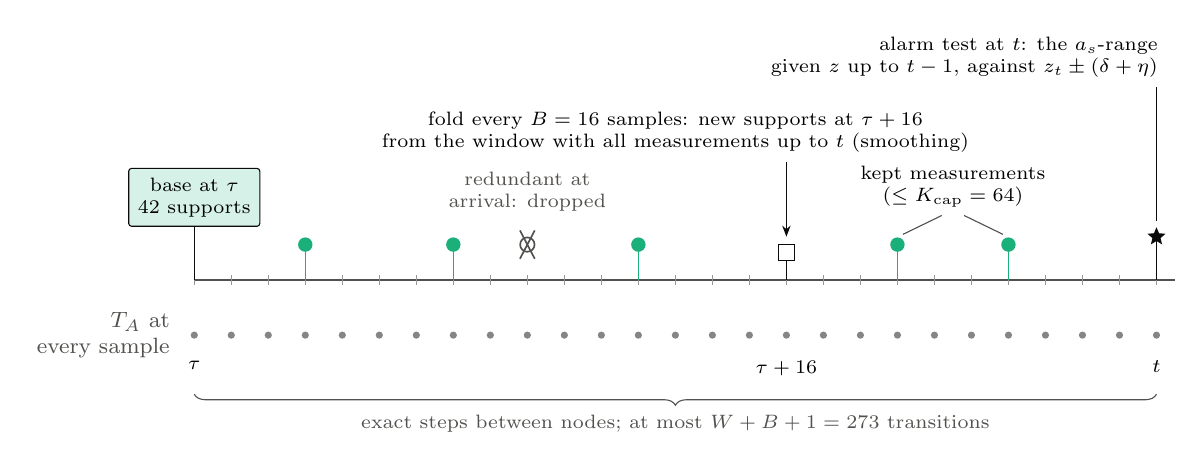
\begin{tikzpicture}[x=0.47cm, y=1cm, font=\footnotesize]
% sample axis
\draw[muted, line width=0.4pt] (0,0) -- (26.5,0);
\foreach \i in {0,...,26} \draw[muted!60] (\i,-0.06) -- (\i,0.06);
% T_A at every sample
\foreach \i in {0,...,26} \fill[muted!70] (\i,-0.7) circle (1.3pt);
\node[anchor=east, muted, align=right] at (-0.4,-0.7) {$T_A$ at\\every sample};
% nodes: base, kept measurements, the fold target, the current sample
\node[draw=ink, fill=cWM!18, rounded corners=1pt, minimum width=1.25cm, minimum height=0.62cm, align=center,
      font=\scriptsize] (base) at (0,1.05) {base at $\tau$\\42 supports};
\draw[ink] (0,0) -- (base.south);
\foreach \i in {3,7,12,19,22} {\fill[cWM] (\i,0.45) circle (2.6pt); \draw[cWM, line width=0.5pt] (\i,0) -- (\i,0.37);}
\draw[muted, line width=0.6pt] (9,0.45) circle (2.6pt);
\draw[muted, line width=0.6pt] (8.8,0.27) -- (9.2,0.63) (8.8,0.63) -- (9.2,0.27);
\node[anchor=south, muted, font=\scriptsize, align=center] at (9,0.75) {redundant at\\arrival: dropped};
\node[anchor=south, font=\scriptsize, align=center] at (20.5,0.8) {kept measurements\\($\le K_{\mathrm{cap}} = 64$)};
\draw[muted, line width=0.4pt] (20.2,0.82) -- (19.15,0.58);
\draw[muted, line width=0.4pt] (20.8,0.82) -- (21.85,0.58);
\draw[ink, line width=0.6pt] (16,0) -- (16,0.35);
\node[draw=ink, fill=white, minimum size=6pt, inner sep=0pt] at (16,0.35) {};
\node[anchor=north, font=\scriptsize] at (16,-0.9) {$\tau+16$};
\node[anchor=north, font=\scriptsize] at (0,-0.9) {$\tau$};
\node[anchor=north, font=\scriptsize] at (26,-0.9) {$t$};
% the current sample: the alarm test
\draw[ink, line width=0.6pt] (26,0) -- (26,0.55);
\node[star, star points=5, star point ratio=2.2, fill=ink, inner sep=1.1pt] at (26,0.55) {};
\node[anchor=south east, align=right, font=\scriptsize] at (26.3,2.45) {alarm test at $t$: the $a_s$-range\\given $z$ up to $t-1$, against $z_t\pm(\delta+\eta)$};
\draw[ink, line width=0.4pt] (26,0.75) -- (26,2.45);
% the fold: smoothing uses every measurement up to t
\draw[-{Stealth[length=4pt]}, ink, line width=0.5pt] (16,1.5) -- (16,0.55);
\node[anchor=south, align=center, font=\scriptsize] at (13,1.5) {fold every $B=16$ samples: new supports at $\tau+16$\\from the window with all measurements up to $t$ (smoothing)};
% the window length
\draw[decorate, decoration={brace, mirror, amplitude=4pt}, muted] (0,-1.45) -- (26,-1.45)
  node[midway, below=4pt, muted, font=\scriptsize] {exact steps between nodes; at most $W+B+1 = 273$ transitions};
\end{tikzpicture}

\caption{The window of WM between two folds (schematic, not to scale). The states $(a_c, a_s)$ appear at the nodes
only: the base at $\tau$, the kept measurements, $\tau+16$ and the current sample; $T_A$ appears at every sample.}
\label{fig:window}
\end{figure}

Between nodes the steps are exact:
$x_b = M^L x_a + \sum_{k<L} M^k e_3 w_{b-1-k}$, with every $|w_j|\le\rho$ explicit. $M^L$ and $M^k e_3$ are the exact
powers of the exact model, each rounded once. The states $(a_c, a_s)$ appear at the nodes only ($\tau$, the kept
measurements, $\tau+16$ and the objective sample) and $T_A$ at every sample. Between nodes, $a_c$ and $a_s$ stay in the
box by convexity, so only the box rows of $T_A$ are needed. Apart from dropped measurements, the window is exact.

A measurement redundant at arrival is dropped. Above $K_{\mathrm{cap}}$ kept measurements, the one inactive longest is
evicted. Both only remove constraints.

The alarm at $t$ uses the $a_s$-range of the window given $z$ up to $t-1$. WM flags only when a \emph{certified} bound
separates it from $[z_t-\delta-\eta,\ z_t+\delta+\eta]$, with $\eta = 10^{-9}$\,\degC\ and the slab rounded outward. A
primal value that points to an alarm the certificate cannot prove raises nothing; $z_t$ is then dropped.

Every $B = 16$ samples the base is folded from $\tau$ to $\tau+16$. Each of the 42 new supports is the maximum of
$d_i\cdot x_{\tau+16}$ over the window \emph{with every measurement up to the current sample $t$}, raised to at least
its certified bound and then clamped. This is the smoothing rule: the new base carries what later measurements say
about the past state. The filtering rule would use the measurements up to $\tau+16$ only.

$\eta$ encloses the floating-point error of the data. The simulator computes $z$ from two binary64 simulations; an a
priori bound puts the data of every healthy run within \sci{5}{-11}\,\degC\ of data that an admissible run of the exact
model explains with $|v|\le\delta$. $\eta$ is 20 times that.
% src: FREEZE-V2.md section 1 (window LP, fold, eta and its a priori bound); FREEZE-V3.md section 1

\subsection{Certificates}\label{sec:cert}

Every alarm bound and every fold bound is a weak-duality bound computed from the solver's multipliers, with every
variable boxed, the floating-point rounding of the bound's own evaluation bounded explicitly, and the rounding of each
LP coefficient enclosed (each is its exact value rounded once). So the bound holds for the LP with exact coefficients,
whatever the solver's tolerance \citep{neumaier2004,jansson2004}. With every variable boxed it holds for \emph{any}
multiplier vector: a solver stopped early gives a looser bound, never an unsound one. The floating-point model is IEEE
binary64 with rounding to nearest and gradual underflow; a product's error beyond the relative model is at most
$2^{-1075}$, and the bound includes that term.

An audit variant evaluates every bound again in exact rational arithmetic. Over all development rows, 3,548,402 bounds
were audited with no violation; the smallest slack was \sci{8.2}{-16}\,\degC. Under simulated solver failures a further
12,572,172 bounds, 425,757 of them fallback bounds, were audited with no violation.
% src: FREEZE-V2.md section 1 "The certificate"; FREEZE-V3.md section 1 floating-point model; DIAG-3-RESULTS.md AF1
% (3,548,402, 8.2e-16) and amendment 10 R3 table (a, b 4,319,122 each, e 3,933,928; implied 39,033 + 386,724)

\begin{proposition}[soundness of WM]\label{prop:wm}
Under the model, WM never flags an admissible record and never flags before $\tstar$, and every flag carries a
certificate.
\end{proposition}
\begin{proof}[Proof sketch]
Let $\mathfrak{X}(t\mid t-1)$ be the explanations of the measurements up to $t-1$ under the exact model, as states at
$t$, with slabs $\delta+\eta$. The window LP with exact coefficients contains $\mathfrak{X}$ when its base at $\tau$
contains the projection of the explanations at $\tau$: its rows are the model's dynamics, the $a_c$ and $a_s$ boxes
hold by convexity, and the $w$ and $T_A$ boxes are the model's. The certificate bounds the ideal window, not the
solver's rounded one. The start is the template's start. Dropping and evicting only remove constraints. Each fold
support is at least the maximum over the ideal window and the clamps hold for every reachable state, so the new base
contains the explanations at $\tau+16$. An alarm needs a certified separation. The full proof, checked line by line
against the code, is in the repository \tocheck{decide whether it goes into an appendix}.
\end{proof}

\subsection{When the solver does not solve}\label{sec:fallback}

Every LP of WM has two outcomes: \emph{solved} (status optimal, after at most three attempts: dual simplex without
presolve, interior point without presolve, dual simplex with presolve) or \emph{failed} (any other status, an exception
from the solver call, or an answer that is not finite). WM never uses a value from a failed LP. A solver's
``infeasible'' is one more failure, not a proof: an alarm needs a certified separation. The fallbacks are outer bounds
(Table~\ref{tab:fallback}).

\begin{table}[ht]
\centering\small
\caption{Fallbacks of WM when an LP fails.}\label{tab:fallback}
\begin{tabular}{>{\raggedright}p{0.24\linewidth}>{\raggedright}p{0.42\linewidth}>{\raggedright\arraybackslash}p{0.24\linewidth}}
\toprule
failed LP & fallback & why it is sound\\
\midrule
one side of the $a_s$-range & that side's box bound; $z_t$ not kept & the box contains every state\\
one side of the alarm certificate & that side's box bound & the same\\
one direction of a fold & the certified maximum over $P_J\cap\text{box}$, $J$ the solved faces of the same fold; if
that LP in three variables fails too, the a priori clamp & the window's states lie in $P_J\cap\text{box}$\\
every direction of a fold & reset: base $=$ the a priori clamps, no kept measurements, $\tau \mathrel{+}= B$ & the
clamps hold under the exact model\\
\bottomrule
\end{tabular}
\end{table}

This path was added after the failure of Section~\ref{sec:val2}. Its tests are in Section~\ref{sec:inject}.
% src: FREEZE-V3.md section 1 tables

\section{Protocol}\label{sec:protocol}

All development (design, diagnosis, tuning) used seeds 430000--430099. Validation seeds 440000--440999 were reserved,
and the generator refuses them unless a freeze record is approved and its manifest matches. Each validation followed
the same order:
\begin{enumerate}
\item A freeze document fixes the hypothesis, the candidate, the scoring rules and the seed block, and a manifest pins
  every file the run uses by sha256.
\item The full pipeline is rehearsed on development seeds.
\item A commit that changes only the document's status line approves it. The runner refuses to start without that
  line, a matching manifest, a clean tree and the fixed environment.
\item The run generates the block once; the scorer applies the fixed rules in a fixed order: integrity, then soundness
  (an alarm on an admissible run, an alarm before $\tstar$, or an uncertified alarm is a FAIL), then completeness
  (undetermined fault runs at most 1\,\%), then misses and the target.
\item Nothing is rerun except after an infrastructure failure as defined in advance; the verdict is recorded as it
  came out, with a dated record.
\end{enumerate}
Every score was reproduced byte for byte on a second machine. The scores of validations 2 and 3 were also reproduced by
an independent scorer written from the rules alone, using only the Python standard library. Each block was used once. A failed candidate is not repaired on its
block: a new candidate needs a new freeze and the next unused block. The environment was CPython 3.12.13, numpy 2.5.5,
scipy 1.18.1 and HiGHS 1.12.0.
% src: FREEZE-V1/V2/V3.md; RECORD-2026-11-19 and -21 "Provenance"

\section{Results}

\subsection{Development: loss against memory}

Table~\ref{tab:dev} gives development results only (1,081 certified detection events), not a validation. Figure~\ref{fig:memory} places these monitors, and the validated ones, by the numbers they keep.

\begin{figure}[t]
\centering
% Figure: D_paired against memory. Data: figdata/fig1_*.dat (paper/figures/make_data.py, fig1).
\begin{tikzpicture}
\begin{semilogxaxis}[paperaxis,
  width=0.92\linewidth, height=6.2cm,
  xmin=1.6, xmax=170, ymin=-0.14, ymax=1.12,
  xtick={2,16,42,60,87,107}, xticklabels={2,16,42,60,87,107},
  minor xtick={}, ytick={0,0.2,0.4,0.6,0.8,1},
  xlabel={numbers kept between samples (log scale)},
  ylabel={$\Dp$},
  legend style={at={(0.03,0.97)}, anchor=north west},
  legend cell align=left]
% the development curve, in memory order
\addplot[muted!55, line width=0.5pt, forget plot] table[x=mem, y=D] {figdata/fig1_dev.dat};
% development points: filled; validation points: open
\addplot[only marks, mark=*, mark size=2.4pt, cIM, forget plot]
  table[x=mem, y=D, restrict expr to domain={\thisrow{fam}}{0:0}] {figdata/fig1_dev.dat};
\addplot[only marks, mark=square*, mark size=2.2pt, cTS, forget plot]
  table[x=mem, y=D, restrict expr to domain={\thisrow{fam}}{1:1}] {figdata/fig1_dev.dat};
\addplot[only marks, mark=diamond*, mark size=2.8pt, cWM, forget plot]
  table[x=mem, y=D, restrict expr to domain={\thisrow{fam}}{2:2}] {figdata/fig1_dev.dat};
\addplot[only marks, mark=square, mark size=3.6pt, cTS, line width=0.8pt, forget plot]
  table[x=mem, y=D, restrict expr to domain={\thisrow{fam}}{1:1}] {figdata/fig1_val.dat};
\addplot[only marks, mark=diamond, mark size=4.2pt, cWM, line width=0.8pt, forget plot]
  table[x=mem, y=D, restrict expr to domain={\thisrow{fam}}{2:2}] {figdata/fig1_val.dat};
% legend entries for the two data sets (ink markers)
\addlegendimage{only marks, mark=*, mark size=2.2pt, ink}
\addlegendentry{development (1,081 events)}
\addlegendimage{only marks, mark=o, mark size=3pt, ink, line width=0.8pt}
\addlegendentry{validation (fresh blocks)}
% direct labels (layout only; values are in the data files)
\node[lab, anchor=north west] at (axis cs:2.1,-0.02) {IM (reference)};
\node[lab, anchor=north] at (axis cs:16,0.10) {inv4p};
\node[lab, anchor=west] at (axis cs:46,0.38) {TS};
\node[lab, anchor=east] at (axis cs:57,0.66) {$W=64$};
\node[lab, anchor=south east] at (axis cs:69.5,0.825) {$W=128$};
\node[lab, anchor=north west] at (axis cs:78,0.815) {$W=192$};
\node[lab, anchor=south east] at (axis cs:85,1.0) {$W=256$};
\node[lab, anchor=north west] at (axis cs:109,0.985) {WM};
\end{semilogxaxis}
\end{tikzpicture}

\caption{$\Dp$ against the numbers a monitor keeps between samples. Filled markers: development (1,081 certified
events); open markers: validation (inv4p and TS on validation 1, WM on validation 3). For a window the count is the 42
supports of its base plus the largest number of measurements it kept on that data; their sample indices, $\tau$ and
the LP workspace are not counted. IM is the reference, with $\Dp = 0$ by definition.}
\label{fig:memory}
\end{figure}

\begin{table}[ht]
\centering\small
\caption{Development: $\Dp$ against the memory of the monitor.}\label{tab:dev}
\begin{tabular}{lllll}
\toprule
monitor & state & $\Dp$ & misses & detections at $\tstar$\\
\midrule
template TS only & 42 numbers & 0.386 & 4 & 897\\
window $W = 64$ & $\le18$ kept & 0.643 & 0 & 1037\\
window $W = 128$ & $\le28$ kept & 0.815 & 0 & 1063\\
window $W = 192$ & $\le35$ kept & 0.824 & 0 & 1073\\
window $W = 256$ & $\le45$ kept & 0.9992 & 0 & 1079\\
\bottomrule
\end{tabular}
\end{table}

The curve is not smooth: between $W = 192$ and 256 the gain comes from a few runs with slow drift whose separating
information lies far back. On 430010 (drift 0.0005\,\degC/s, ramp ambient), $W = 192$ detects at 3,449 and $W = 256$ at
$\tstar = 695$. Figure~\ref{fig:trace} shows this run. With a cap of 64, development data never kept more than 45 measurements, so nothing was evicted. Caps of
40 and 32 detected identically on all 1,320 rows, with 420 and 21,821 evictions.
% src: DIAG-3-RESULTS.md "size-loss curve"; amendment 6 part 2 (K1, K2, K = 40 table, K = 32)
% src (figures): paper/figures/make_data.py -> figdata/figures.json; inv4p DEV D_paired 0.147 scored there

\paragraph{Smoothing against filtering.} On the four diagnosis runs, the filtering fold never recovers run 430027 at
any $W$ (it stays at 1,429 against $\tstar = 579$), and recovers 430010 only to 3,449 at $W = 256$ ($\tstar = 695$). The
smoothing fold detects both at $\tstar$ (at $W = 128$ and $W = 256$). \pending{B5, the forward window, on the validation
block.}
% src: DIAG-3-RESULTS.md phase 1 tables

\begin{figure}[t]
\centering
% Figure: development run 430010 (drift 0.0005 C/s, E0, ramp). Data: figdata/fig2_trace.dat (make_data.py, fig2).
% Columns: k, z (shifted), and the a_s-range each monitor tests z_k against (lo, hi). delta = 0.3.
\begin{tikzpicture}
\begin{groupplot}[group style={group size=1 by 2, vertical sep=1.6cm},
  paperaxis, width=0.92\linewidth, unbounded coords=jump]
% (a) the upper edge of the acceptance band, hi + delta, near t*
\nextgroupplot[height=5.2cm, xmin=670, xmax=700, ymin=-0.80, ymax=-0.69, restrict x to domain=660:710,
  restrict y to domain=-1.2:-0.4, ylabel={$^\circ$C (shifted)}, xlabel={sample $k$},
  title={(a) upper edge $\bar a_s+\delta$ of the band each $z_k$ is tested against},
  legend style={at={(0.98,0.03)}, anchor=south east}, legend cell align=left]
\addplot[only marks, mark=*, mark size=1pt, muted!70] table[x=k, y=z] {figdata/fig2_trace.dat};
\addlegendentry{measurement $z_k$}
\addplot[cIM, densely dashed, line width=0.9pt] table[x=k, y=imtop] {figdata/fig2_trace.dat};
\addlegendentry{IM}
\addplot[cTS, dotted, line width=1.1pt] table[x=k, y=tstop] {figdata/fig2_trace.dat};
\addlegendentry{TS}
\addplot[cWM, line width=0.9pt] table[x=k, y=wmtop] {figdata/fig2_trace.dat};
\addlegendentry{WM}
\addplot[only marks, mark=o, mark size=3.2pt, ink, line width=0.6pt, forget plot,
  restrict expr to domain={\thisrow{k}}{695:695}] table[x=k, y=z] {figdata/fig2_trace.dat};
\node[lab, anchor=south east] at (axis cs:694.4,-0.7) {$z_{695}$: above WM's edge only};
% (b) the width of the range over the whole record, as a running median
\nextgroupplot[height=5.2cm, ymode=log, xmin=0, xmax=3600, ymin=0.02, ymax=0.3,
  ylabel={width ($^\circ$C)}, xlabel={sample $k$},
  title={(b) width of the $a_s$-range, median over 61 samples},
  ytick={0.02,0.05,0.1,0.2}, yticklabels={0.02,0.05,0.1,0.2}]
\addplot[cIM, densely dashed, line width=0.8pt] table[x=k, y=immed] {figdata/fig2_trace.dat};
\addplot[cTS, dotted, line width=1pt] table[x=k, y=tsmed] {figdata/fig2_trace.dat};
\addplot[cWM, line width=0.8pt] table[x=k, y=wmmed] {figdata/fig2_trace.dat};
\draw[muted, line width=0.4pt, dashed] (axis cs:496,0.02) -- (axis cs:496,0.3);
\draw[muted, line width=0.4pt, dashed] (axis cs:695,0.02) -- (axis cs:695,0.3);
\draw[muted, line width=0.4pt, dashed] (axis cs:3575,0.02) -- (axis cs:3575,0.3);
\node[lab, anchor=north east, align=right] at (axis cs:490,0.29) {fault\\onset 496};
\node[lab, anchor=north west, align=left] at (axis cs:700,0.29) {WM flags\\at $t^\ast=695$};
\node[lab, anchor=north east, align=right] at (axis cs:3565,0.29) {IM and TS\\flag at 3575};
\node[lab, anchor=south] at (axis cs:2300,0.125) {IM (dashed), TS (dotted)};
\node[lab, anchor=north] at (axis cs:130,0.029) {WM};
\end{groupplot}
\end{tikzpicture}

\caption{Development run 430010 (drift 0.0005\,\degC/s from sample 496, E0, ramp ambient; $\tstar = 695$).
(a)~The upper edge of the band each measurement is tested against, $\bar a_s+\delta$, with $\bar a_s$ the top of the
monitor's $a_s$-range given the past; a measurement above a monitor's edge is an alarm of that monitor. At sample 695
the measurement lies 0.3\,m\degC\ above WM's edge and about 5\,m\degC\ below the edges of IM and TS. (b)~The width of
the $a_s$-range; WM's curve ends at its alarm.}
\label{fig:trace}
\end{figure}

\subsection{Validation 1: the template tier}

Block 440000--440199 (9,600 runs; 7,201 certified events, 4 undetermined fault runs).

\begin{table}[ht]
\centering\small
\caption{Validation 1. Seed bootstrap; misses of IM on this block: 24.}\label{tab:val1}
\begin{tabular}{lllllll}
\toprule
 & target & $\Dp$ & bootstrap 95\,\% & misses & later than IM & verdict\\
\midrule
inv4p (16 numbers) & 0.10 & 0.152 & $[0.107, 0.205]$ & 20 & 0 & PASS\\
TS / cyl16p (42 numbers) & 0.25 & 0.387 & $[0.323, 0.452]$ & 16 & 0 & PASS\\
\bottomrule
\end{tabular}
\end{table}

Neither monitor had a soundness finding: no alarm on any of the 2,395 admissible runs. The C float64 builds equal the
Python implementation on all 9,600 runs.
% src: RECORD-2026-11-18-validation.md Verdicts

\subsection{Validation 2: the window tier fails on one LP}\label{sec:val2}

Block 440200--440399. The window (then without the fallback path of Section~\ref{sec:fallback}) reached $\Dp = 0.995$
with no miss (IM missed 14). On one healthy run with edge noise (440243, E0, ramp), one fold LP ended unsolved in HiGHS
in all three attempts at $t = 945$, and the frozen code recorded an uncertified alarm. Under the frozen order, that row
is a soundness violation and an uncertified alarm, and the verdict is \textbf{FAIL} before any accuracy rule is
reached. The accuracy numbers are reported with the failure and are not a validation.

A diagnosis afterwards, outside the scored run, replayed the row deterministically. The failure was confined to one of
the 42 fold directions; the other 41 solved faces bound that direction at $-0.209$\,\degC\ (its previous base bound
was $-0.187$ and its a priori bound 1.683). That observation became the fallback of Section~\ref{sec:fallback}.
% src: RECORD-2026-11-19-validation.md (verdict, diagnosis)

\subsection{Validation 3: the window tier with its fallback path}

Block 440400--440599.

\begin{table}[ht]
\centering\small
\caption{Validation 3: WM with $W = 256$, $B = 16$, $K_{\mathrm{cap}} = 64$. Seed bootstrap; misses of IM on this
block: 27.}\label{tab:val3}
\begin{tabular}{lllllll}
\toprule
 & target & $\Dp$ & bootstrap 95\,\% & misses & uncertified & verdict\\
\midrule
WM / F3 & 0.80 & 0.9952 & $[0.9899, 0.9995]$ & 0 & 0 & PASS\\
\bottomrule
\end{tabular}
\end{table}

Figure~\ref{fig:cells} shows where the lag of each monitor lies.

\begin{figure}[t]
\centering
% Figure: validation 3, lag per fault cell, IM against WM. Data: figdata/fig4_cells.dat (make_data.py, fig4).
% Rows (i): jump 0.5, jump 0.2, stuck, noise x2, gain 0.01, drift 0.02, 0.005, 0.002, 0.001, 0.0005 (C/s).
\begin{tikzpicture}
\begin{semilogxaxis}[paperaxis,
  width=0.86\linewidth, height=7.2cm,
  xmin=0.5, xmax=1e6, ymin=-0.6, ymax=9.6, y dir=reverse,
  ytick={0,...,9},
  yticklabels={jump 0.5\,$^\circ$C, jump 0.2\,$^\circ$C, stuck, noise $\times2$, gain 1\,\%, drift 0.02, drift 0.005,
               drift 0.002, drift 0.001, drift 0.0005},
  xtick={1,10,100,1000,10000,100000,1000000},
  xlabel={lag summed over the cell's certified events (s; misses count $N-t^\ast$)},
  ymajorgrids=true, xmajorgrids=true,
  legend style={at={(0.08,0.03)}, anchor=south west}, legend cell align=left]
\addplot[only marks, mark=*, mark size=2.4pt, cIM] table[x=im, y=i] {figdata/fig4_cells.dat};
\addlegendentry{IM}
\addplot[only marks, mark=diamond*, mark size=3pt, cWM,
  restrict expr to domain={\thisrow{wm}}{1:1e9}] table[x=wm, y=i] {figdata/fig4_cells.dat};
\addlegendentry{WM}
% WM's lag is 0 in seven cells: open diamonds at the left edge
\addplot[only marks, mark=diamond, mark size=3pt, cWM, line width=0.7pt,
  restrict expr to domain={\thisrow{wm}}{-1:0.5}] table[x expr=0.7, y=i] {figdata/fig4_cells.dat};
\addlegendentry{WM, lag 0 (left edge)}
% IM's misses (selective labels)
\node[lab, anchor=west] at (axis cs:40000,1) {8 missed};
\node[lab, anchor=west] at (axis cs:75000,8) {2 missed};
\node[lab, anchor=west] at (axis cs:125000,9) {17 missed};
\end{semilogxaxis}
\end{tikzpicture}

\caption{Validation 3: the lag of IM and WM in each fault cell, summed over the cell's certified events, with a miss
counted as $N-\tstar$ (log scale). WM's lag is 0 in seven cells (open diamonds at the left edge). IM's 27 misses are
in the three labelled cells.}
\label{fig:cells}
\end{figure}

\begin{itemize}
\item No soundness finding. 7,255 certified events; 7,243 detected exactly at $\tstar$ (IM: 5,257). Lag p90 0\,s and
  maximum 212\,s (IM: 55\,s and 2,215\,s). No run was later than IM.
\item 7,258 alarms, all certified, the largest certified margin $-0.0147$\,m\degC; three of them on fault runs the
  oracle left undetermined.
\item The remaining lag sits in three cells: drift 0.0005 and 0.001\,\degC/s with ramp ambient, and drift
  0.002\,\degC/s with rw ambient. Drifts carry 99.8\,\% of IM's lag.
\item The fallback path never ran on this block. WM solved 53,968,652 LPs with 722 retries (on 320 runs), and every LP was solved
  within its three attempts. The validation supports the window's accuracy and the soundness of its normal path; the
  fallback path rests on its proof and on Section~\ref{sec:inject}.
\item At most 65 measurements kept, at most 445 LP rows and 679 variables.
\end{itemize}
% src: RECORD-2026-11-21-validation.md

\subsection{The fallback path under injected solver failures}\label{sec:inject}

A separate preregistered test injected solver failures into WM on 1,200 fresh runs (25 seeds of a separate namespace)
in six settings: 1\,\% and 10\,\% of the LPs of fold directions; 1\,\% of the $a_s$-range and certificate LPs; every
direction of every fourth fold; 10\,\% of fold directions together with every $P_J$ LP; every upper certificate LP.
All criteria held in every setting: no alarm on an admissible run, none before $\tstar$, every alarm certified, at most
65 kept measurements, the fallback counters equal to the injection log, and every fallback path reached (for example
375,725 implied $P_J$ bounds and 22,600 full resets). The exact audit of two settings checked 7,300,179 bounds with no
violation.

The cost was in detection. With 1\,\% and 10\,\% fold failures nothing was missed; one detection in the 10\,\% setting
came 45 samples later than without injection. With 1\,\% of the $a_s$-range and certificate LPs failing, 22 detections
came later (median 6 samples), nothing was missed and $\Dp$ was 0.977; 14 events that IM detects were detected after
IM. With every fourth fold reset, 30 events were missed and $\Dp$ was $-5.21$; with every upper certificate failing,
174 were missed and $\Dp$ was $-29.24$. In these two settings WM was later than IM, or missed, on 232 and 752 of the
events that IM detects.
% src: RECORD-2026-11-21-fb.md (settings table: later, missed, D_paired, later than v2 or missed where v2 detects);
% settings = FB-PLAN.md table

\paragraph{The solver's process.} In the runs above the LPs run in WM's own process. A solver that ends its process (as
the interior-point solver did in 8 of the oracle's 117,606 attempts in validation 3, by a segmentation fault) would end
the run before any fallback could see it. In a variant, WM's LPs run in a child process that persists across LPs; if
the child ends or does not answer in 120\,s, it is replaced and the attempt counts as failed, so the fallbacks of
Section~\ref{sec:fallback} apply. Without injection the variant equals WM in every recorded field but time on 6 development
rows. On the 1,400 development rows the child then ended itself before 15,320 LPs, in all three attempts of each (half
by exit, half by a segmentation fault; two per thousand fold LPs, one per thousand $a_s$-range LPs, a fifth of the LPs
of implied bounds and half of the certificate LPs). Every run completed. No alarm came on an admissible run or before
$\tstar$, every alarm was certified, the fallback counters equalled the injection log on every row, and at most 65
measurements were kept. Again the cost was in detection: 497 detections came later (median 5 samples) and 3 events
with slow drift were missed; none came earlier. Two documented paths lead there: an alarm whose certificate cannot be
computed is not raised, and a measurement checked against a failed $a_s$-range LP is not kept. Their shares were not
computed.
% src: RECORD-2026-11-21-iso.md; ISOLATION-PLAN.md section 2 (rates); RECORD-2026-11-21-validation.md lines 193-200
% (8 of 117,606 oracle attempts, all highs-ipm)

\subsection{Precision and microcontrollers}\label{sec:mcu}

\paragraph{float32 builds.} Built with float32 tables, the template state was sound on the first validation block,
including the 800 healthy runs with noise exactly at $\pm\delta$. But TS in float32 reached $\Dp = 0.212$ (target 0.25)
and was later than IM on 52 runs; inv4p in float32 reached 0.004 with 28 misses and was later than IM on 130 runs.
Theorem~\ref{thm:dom} holds in exact arithmetic, not in float32. Neither float32 build was the object of a hypothesis.
% src: RECORD-2026-11-18-validation.md lines 92-105

\paragraph{ESP32 with float64 tables.} The C implementation of TS with the validated float64 tables ran on an ESP32
(240\,MHz) on all 1,400 development rows, 5,040,000 samples. On every sample the alarm flag and a 16-byte hash of the
full state equalled the PC build's (preregistered; negative controls detected a change of $10^{-6}$ in one input and a
single flipped bit). Per sample, on the 322 rows that never flag (after a flag the state stops): 3.63\,ms median,
4.56\,ms maximum. On four earlier rows a float32 build took 0.49\,ms median against 3.72 to 3.74\,ms for float64.
% src: MCU-NOTES 2d, 2e

\paragraph{8-bit AVR with float32 tables.} On an ATmega328P (16\,MHz, 2\,KB SRAM) the float32 build used at most 602
bytes of SRAM and 28,064 bytes of flash, at 74 to 76\,ms per sample. On 30 preregistered development rows its first
flagged sample equalled the PC float32 build's on every row. Its state is not equal bit for bit: the board's binary64
is faithful but not correctly rounded, and the largest measured difference in a support was \sci{7.2}{-7}\,\degC. That
is far below the margins at which the test changes its answer, but the pads do not cover it by construction.
% src: MCU-NOTES 2c, 2f

\paragraph{The C state against the exact model.} A check in exact rational arithmetic found two gaps in the frozen C
state. (i) The command part $S$ is computed in binary64 and no pad covers its rounding: the frozen C state is sound
against the exact model for $|v|\le\delta-\varepsilon$, with $\varepsilon = \sci{4.85}{-13}$\,\degC\
(\sci{9.9}{-13}\,\degC\ on the AVR). (ii) Two start supports were \sci{1.11}{-16}\,\degC\ short; the first step absorbs
the shortfall. A revised C state closes both by construction, with the slab $\delta+\eta$ and exact start sums, so that
it is sound for $|v|\le\delta$. Preregistered checks accepted it: the same first flag as the frozen C state on all
1,400 development rows, equality bit for bit with its PC build on the ESP32 over 5,040,000 samples, and the same first
flag as its PC build on the AVR on 30 rows. On development data the fix cost no detection. It is not validated on
fresh seeds. The same check of the validated Python template is open at the $10^{-21}$ level (two rate pads
\sci{2.1}{-21}\,\degC\ below their exact value).
% src: MCU-NOTES 2g, 2h; C1-PLAN.md

\subsection{Baselines}\label{sec:baselines}

\pending{B1 constrained zonotopes \citep{scott2016}, B2 zonotopes with strip intersection \citep{alamo2005}, B3 a
zonotopic observer with constant gain \citep{combastel2015}, B4 an interval observer, B5 the forward window (in the
style of \citealt{kesavan2001}), tuned on development rows and frozen before the block run on the window's validation
block (BASELINE-PLAN.md). Report memory against $\Dp$ and misses, with WM and TS.}

\subsection{How much the results lean on the ambient box}\label{sec:ambient}

A descriptive study on development seeds, preregistered without pass or fail, asked two questions.

\paragraph{A wider assumed box.} On the 1,320 development rows (true ambient within $[23, 27]$), widening the assumed box
to $[22, 28]$ multiplied IM's lag against the $\tstar$ of the frozen box by 2.9 and TS's by 4.1; to $[21, 29]$, by 3.5
and 5.2. Misses rose from 8 to 32 and 55 (IM) and from 4 to 28 and 51 (TS). The whole increase is in the three slowest
drift cells; jumps, faster drifts, gain, noise and stuck faults do not depend on the box. TS stays about 17,500\,s of
lag ahead of IM at every box, so its relative gain falls from 40\,\% to 14\,\% and 11\,\%. No monitor flagged an
admissible row or flagged before $\tstar$, at any box. These lags mix two losses: what a monitor discards, and what the
weaker assumption no longer gives (the exact detector is later too; its $\tstar$ for the wider boxes was not computed).
WM was not run with a wider box, since the box enters its LP, certificates and fallbacks.

\paragraph{Broken assumptions, healthy sensor.} With the frozen assumptions and healthy sensors, an ambient rate twice
the bound caused no alarm in any monitor on 60 runs. A rate five times the bound caused certified alarms of WM on 4 of
60 runs (two paths, both arms) and none of IM or TS; WM keeps the most information of the three and was the only one to
prove these violations. A 1\,\degC\ step in the ambient was flagged by all three on every run, 1 to 10 samples after the
step. An ambient path starting outside the box was flagged by all three within 3 samples of the start; a slow excursion
out of the box was not tested. The sensor was healthy in every run of this part, so each of these alarms reports a
broken assumption.
% src: RECORD-2026-11-21-ambient.md; results/v3/ambient/amb-443d8b30-mac/ (summary.json, report.json)

Development data had already shown why detection of slow drift depends on the box. In those cells the alarm often
comes when $z$ exceeds the top of the box plus $\delta$, so that every healthy explanation has to push $T_A$ against
the wall: on every development run where a window variant without box rows of $T_A$ between nodes was later than the
full window, $z$ reached 2.22 to 2.30 (shifted units) in the 256 samples before $\tstar$.
% src: FREEZE-V2.md section 1 "The ambient box matters to the result" (DIAG-3 amendment 5)

\section{What went wrong}\label{sec:wrong}

The records keep every failure. These changed the method:
\begin{enumerate}
\item One unsolved LP failed a validation (Section~\ref{sec:val2}). The window's rules said an unsolved fold is an
  uncertified alarm; the rule was sound but incomplete. The fallback path of Section~\ref{sec:fallback} replaced it and
  was tested on a new block and under injection.
\item The binary64 model was not the exact model. The first window LP and the template tables were built against the
  binary64 matrix, whose rows do not sum to one, and against data with their own simulation error. A later revision
  moved every exact computation to the simulator's recurrence with its parameters read as rationals, and added $\eta$
  for the data. Before that revision the template state came within \sci{1.9}{-14} to \sci{3.0}{-14}\,\degC\ of a
  false alarm on 48 of the 80 development runs with edge noise: observed, not proved impossible.
\item The C state had two gaps, of order $10^{-13}$ and $10^{-16}$ (Section~\ref{sec:mcu}), found by a check written
  after the microcontroller runs. One more, at \sci{2.1}{-21} in the Python template, is still open.
\item In float32 the template loses its dominance over IM (Section~\ref{sec:mcu}). The development rehearsal before
  the first validation already showed it: the float32 build of the 16-number template detected 430098 (drift
  0.002\,\degC/s, rw) at 906, 240\,s after IM. The validation was then written to claim Theorem~\ref{thm:dom} for
  float64 only.
\item Three claims were corrected after review. An earlier note read as if a drift rate within $\rho$ and room in the
  box were enough for a healthy twin (Proposition~\ref{prop:twin} gives a counterexample). Another said that ``no
  alarm'' means an admissible explanation exists; that holds for the exact test only, not for an outer approximation.
  ``A measurement redundant at arrival stays redundant'' is false once the base is folded: a looser base can make it
  active again, so dropping it is sound and only empirically lossless.
\item When the compressed window was first checked against the dense window LP, the two disagreed by
  \sci{2.8}{-6}\,\degC\ on one support. The error was in the reference: the dense LP had been solved loosely (equality
  residual \sci{6.2}{-5}), and the compressed window was exact to $10^{-11}$.
\end{enumerate}
% src: RECORD-2026-11-19-validation.md; FREEZE-V2.md section 1; RECORD-2026-11-18-validation.md addendum; MCU-NOTES 2g;
% V3_NOTES sections 4, 8; DIAG-3-RESULTS.md (amendment 3, C0); item 4 = FREEZE-V1.md section 8 rehearsal

\section{Related work}\label{sec:related}

\paragraph{Set-membership fault detection.} \citet{puig2010} reviews detection by consistency with unknown but
bounded uncertainty. Consistency tests with parallelotopes \citep{ingimundarson2005}, with zonotopes
\citep{ingimundarson2009} and with constrained zonotopes \citep{scott2016} give sound detectors with bounded complexity;
set-valued observers do the same for LTV and LPV systems \citep{rosa2010,silvestre2017}. Interval observers are the
other main family \citep{pourasghar2019,tang2019}. \citet{saccani2022} apply a set-based approach to thermal faults of a
lithium-ion cell and report earlier detection than an interval method based on constraint propagation. These works
compare detectors with one another; here every detector is compared with the exact detection time.

\paragraph{Bounded memory and the exact set.} The complexity of the exact set cannot be bounded a priori, which
motivates filters of bounded complexity \citep{sznaier2011,blanchini2012}. \citet{casini2024} plot the volume of
estimators with bounded memory against memory depth relative to the exact feasible set, for state estimation.
\citet{scott2016} compare constrained zonotopes with the exact set on estimation volume, and sweep complexity against
detection time without the exact observer.

\paragraph{Moving windows.} \citet{kesavan2001} detect faults with a moving horizon whose initial set is an outer bound
propagated forward (as summarized by \citealt{ingimundarson2005}; \tocheck{primary text not read}). Set-valued moving
horizon estimation appears in MPC with output feedback \citep{brunner2018,kohler2021} and in distributed estimation
\citep{segovia2022}. The arrival cost of quadratic MHE has filtering and smoothing forms
\citep{rao2001,haseltine2005}; set-membership smoothing exists for state estimation \citep{garulli1999,li2026}. WM's
base update is the smoothing form, used for detection in a bounded window.

\paragraph{Certified LP bounds.} Rigorous bounds from approximate duals with boxed variables are due to
\citet{neumaier2004} and \citet{jansson2004}, reviewed by \citet{guilbeau2017}; they are used in exact MIP
\citep{cook2013} and in program analysis with template polyhedra \citep{wang2021}.

\paragraph{Embedded solvers.} DAQP \citep{arnstrom2022} and EIQP \citep{wu2025} target embedded LPs and QPs with
bounded iteration counts; they are dense, and WM's sparse LP of up to 445 rows and 679 variables does not fit them as
is. Because the certificate holds for any multiplier vector, a solver stopped at an iteration cap would keep WM sound
and cost only delay (Section~\ref{sec:cert}); its worst-case time is not shown.

\section{Limitations and open problems}

\begin{itemize}
\item One plant with known parameters, in simulation, under assumed laws of noise and ambient. With uncertain
  parameters the exact set is no longer convex.
\item The ambient box (c) carries the detection of slow drift (Section~\ref{sec:ambient}). A wrong box can make a
  healthy record inconsistent.
\item WM runs on a desktop with HiGHS. An embedded LP solver with a bounded iteration count is the open step; the
  certificate makes early stopping safe but not free.
\item No worst-case execution time for either tier; the microcontroller times are maxima over the runs shown.
\item WM's fallback path was never exercised on validation seeds; it rests on its proof and on injected failures.
\item The facet count of $X_k$, and a principled minimal template, are open.
\item The undetermined oracle runs (healthy runs with noise exactly at $\pm\delta$, about half of them) are judged by
  ground truth, not by the oracle.
\end{itemize}

\section{Reproducibility}

The code, the frozen documents, the manifests and every record cited are in the project repository \pending{public URL
after release}. Each validation is identified by its approval commit and manifest hash: validation 1, approval
\texttt{8e589911}, manifest \texttt{e8dd60f1\dots}; validation 2, approval \texttt{35b344df}, manifest
\texttt{cc7adffa\dots}; validation 3, approval \texttt{948b46b0}, manifest \texttt{0a40cbdf\dots}.

\section*{Declarations}

Funding: none. Competing interests: none. Use of AI tools: \pending{statement by the author}.

\bibliographystyle{plainnat}
\bibliography{refs}

\end{document}
